
\documentclass[acmsmall,review,screen]{acmart}\settopmatter{printfolios=true,printccs=false,printacmref=false}

\citestyle{acmauthoryear}

\newif\ifWGfourteennumber
\WGfourteennumberfalse


\usepackage[normalem]{ulem}
\usepackage{wrapfig}
\usepackage{minibox}

%% Some recommended packages.
\usepackage{booktabs}   %% For formal tables:
                        %% http://ctan.org/pkg/booktabs
\usepackage{subcaption} %% For complex figures with subfigures/subcaptions
                        %% http://ctan.org/pkg/subcaption
\usepackage{verbatim}


\newif\ifmycopyright\mycopyrightfalse
%\mycopyrighttrue
\setcopyright{none}

\bibliographystyle{ACM-Reference-Format}
%% Citation style
%\citestyle{acmauthoryear}  %% For author/year citations
%\citestyle{acmnumeric}     %% For numeric citations
%\setcitestyle{nosort}      %% With 'acmnumeric', to disable automatic
                            %% sorting of references within a single citation;
                            %% e.g., \cite{Smith99,Carpenter05,Baker12}
                            %% rendered as [14,5,2] rather than [2,5,14].
%\setcitesyle{nocompress}   %% With 'acmnumeric', to disable automatic
                            %% compression of sequential references within a
                            %% single citation;
                            %% e.g., \cite{Baker12,Baker14,Baker16}
                            %% rendered as [2,3,4] rather than [2-4].


%%%%%%%%%%%%%%%%%%%%%%%%%%%%%%%%%%%%%%%%%%%%%%%%%%%%%%%%%%%%%%%%%%%%%%
\usepackage[utf8]{inputenc}
\usepackage[T1]{fontenc}
\usepackage{amsmath,amsthm,amssymb,bm,mathtools}

\usepackage[all]{xy}

% these are useful comments, maybe we should make them footnotes?
\renewcommand{\comment}[2][comment]{{\color{blue}\bf[#1: #2]}}
% uncomment the following line to remove comments
 \renewcommand{\comment}[2][comment]{}

\newcommand{\TODO}[1]{{\color{red}\bf[TODO: #1]}}
\definecolor{VGcolor}{rgb}{0.9 0.2 0.0}
\newcommand{\VG}[1]{{\color{VGcolor}\bf[VG: #1]}}
\definecolor{Kcolour}{rgb}{0.87451 0.5 0.0}
\newcommand{\K}[1]{{\color{Kcolour}\bf[K: #1]}}
%\renewcommand{\TODO}[1]{}

\newcommand{\myparagraph}[1]{\vspace{0.5\baselineskip}\par\noindent{\normalsize\bfseries{#1}}\quad}
\newcommand{\myqs}[1]{\vspace{0.2\baselineskip}\par\noindent{\normalsize\bfseries{#1}}\quad}

\def\elasticquad{\hspace{0em plus 1em}\relax}

\newcommand{\myq}[1]{\vspace{0.2\baselineskip}\par\noindent{\normalsize\emph{#1}}\quad}

\newcommand{\mydemotesturl}[1]{https://cerberus.cl.cam.ac.uk/cerberus?demo/#1}
\newcommand{\mytesturl}[1]{https://cerberus.cl.cam.ac.uk/cerberus?defacto/#1}
\newcommand{\mytestlink}[2]{\href{\mytesturl{#1}}{#2}}
\newcommand{\mylsttestlink}[1]{\mytestlink{#1}{\lstinline{#1}}}

%\newcommand{\mytestlink}[2]{\url{#2}} %\href{\mytesturl{#1}}{\lstinline{#2}}}
% macros for question-tooling generated latex
\newcommand{\myqtquestion}[2]{\myparagraph{#1. #2}}
%\newcommand{\myqtexample}[3]{\myexampleheader{#2}  \url{#3}\lstinputlisting{#1#2}}
\newcommand{\mylistingmargin}{5mm}
\newcommand{\myqtlinkexample}[4]{{\vspace*{-0.5\baselineskip}\par{\noindent\small\hspace*{\mylistingmargin}\lstinline{//} #4\lstinputlisting[showstringspaces=false,xleftmargin=\mylistingmargin,aboveskip=0mm]{tests-hand-edited/#2}\vspace*{-0.25\baselineskip}}}}

\newcommand{\myqtexample}[3]{\myqtlinkexample{#1}{#2}{#3}{{\mylsttestlink{#2}}}}

\newcommand{\myfooexamplename}[1]{\mylsttestlink{#1}}
\newcommand{\myfooexample}[3]{{\vspace*{-0.5\baselineskip}\par{\noindent\small\hspace*{\mylistingmargin}\lstinline{//} \mylsttestlink{#2}\lstinputlisting[showstringspaces=false,xleftmargin=\mylistingmargin,aboveskip=0mm]{#1/#2}\vspace*{0.25\baselineskip}\par}}}

\newcommand{\myfoolinkexample}[4]{{\vspace*{-0.5\baselineskip}\par{\noindent\small\hspace*{\mylistingmargin}\lstinline{//} #4\lstinputlisting[showstringspaces=false,xleftmargin=\mylistingmargin,aboveskip=0mm]{#1/#2}\vspace*{0.25\baselineskip}\par}}}

\newcommand{\mycerbexamplename}[2]{\mytestlink{#2}{\lstinline{#1}}}
\newcommand{\mycerbexample}[4]{{\vspace*{-0.5\baselineskip}\par{\noindent\small\hspace*{\mylistingmargin}\lstinline{//} \mycerbexamplename{#2}{#4}\lstinputlisting[showstringspaces=false,xleftmargin=\mylistingmargin,aboveskip=0mm]{#1/#2}\vspace*{0.25\baselineskip}\par}}}


\usepackage{alltt}

\makeatletter
\newcommand{\manuallabel}[2]{\def\@currentlabel{#2}\label{#1}}
\makeatother

\usepackage[scaled=0.82]{beramono}
\usepackage{listings}
\lstset{basicstyle=\renewcommand{\baselinestretch}{0.9}\tt\small}
%\lstset{basicstyle=\tt} 
\lstset{language=c}
%\lstset{numbers=left}
% \lstset{basicstyle=\ttfamily} 
% \lstset{basicstyle=\footnotesize\ttfamily} 
\lstset{keywordstyle=\bfseries}



%%%%%%%%%%%%%%%%%%%%%%%%%%%%%%%%%%%%%%%%%%%%%%%%%%%%%%%%%%%%%%

%\usepackage{tikz}
%\usepackage{pgfplots}

\newenvironment{tightenumerate}{%
\begin{enumerate}%
\setlength{\partopsep}{0pt}%
\setlength{\itemsep}{1pt}%
\setlength{\parskip}{0pt}%
\setlength{\parsep}{0pt}%
}{\end{enumerate}
}
\newenvironment{vtightenumerate}{%
\begin{enumerate}%
\setlength{\topsep}{0pt}%
\setlength{\partopsep}{0pt}%
\setlength{\itemsep}{1pt}%
\setlength{\parskip}{0pt}%
\setlength{\parsep}{0pt}%
}{\end{enumerate}
}

%\setlength{\leftmargini}{0mm}

\newenvironment{tightitemize}{
% \begin{itemize}
%   \setlength{\labelwidth}{0pt}
%   \setlength{\leftmargin}{0pt}
%   \setlength{\itemsep}{1pt}
%   \setlength{\parskip}{0pt}
%   \setlength{\parsep}{0pt}}{\end{itemize}
% }

% \newenvironment{verytightitemize}{
 \begin{itemize}
   \setlength{\itemsep}{0pt}
   \setlength{\parskip}{0pt}
   \setlength{\leftmargin}{0pt}
   \setlength{\leftmargini}{1.5mm}
   \setlength{\leftmarginii}{3mm}
   \setlength{\leftmarginiii}{4.5mm}
   \setlength{\labelwidth}{1.5mm}
   \setlength{\itemindent}{0mm}
   \setlength{\labelsep}{1.5mm}
   \setlength{\rightmargin}{0pt}
   \setlength{\topsep}{0pt}
   \setlength{\parsep}{0pt}}{\end{itemize}
 }

\newenvironment{verytightitemize}{
\begin{list}{\hspace*{-2mm}$\bullet$}{
  \setlength{\itemsep}{1pt}
  \setlength{\topsep}{2pt}
  \setlength{\parskip}{0pt}
  \setlength{\leftmargin}{2mm}
  \setlength{\labelwidth}{0pt}
%  \settowidth{\labelwidth}{$\bullet$}
%  \setlength{\itemindent}{0pt}
  \settowidth{\itemindent}{$\bullet$}
  \addtolength{\itemindent}{0mm}
  \setlength{\parsep}{0pt}}}{\end{list}
}

%%%%%%%%%%%%%%%%%%%%%%%%%%%%%%%%%
\newif\ifWithCharonData\WithCharonDatatrue
\WithCharonDatafalse
\newif\ifWithCharonSome\WithCharonSometrue
\WithCharonSomefalse


%%%%%%%%%%% typesetting of Charon output %%%%%%%%%%%%
\newcommand{\charontt}[1]{\texttt{#1}}
\newcommand{\charonZeroExitCodes}[2]{}
\newcommand{\charonNonZeroExitCodes}[2]{{\color{red}[*** exit codes #1 / #2 ***]}}
\newcommand{\charonSourcesMismatch}{{\color{red}SOURCES MISMATCH}}


% #1  tool instance name
% #2  tool command-line name
% #3  tool args
% #4  compile stderr    
% #5  compile and execute exit codes 
% #6  stdout            
% #7  stderr            
% #8  unused
% #9  execute signals
\newcommand{\charonSameOutcome}[9]{\noindent\textsc{#1:} %
 \ldots as above\\}
\newcommand{\charonSameModuloAddressesOutcome}[9]{\noindent\textsc{#1:} %
 \ldots as above (modulo addresses)\\%
%{}[#5/#8]#9\\\charontt{#4}\charontt{#6}\charontt{#7}%
}
\newcommand{\charonOutcome}[9]{\noindent\textsc{#1:} %
#5#9\\\charontt{#4}\charontt{#6}\charontt{#7}}

% #1  flavour (iso/defacto)
% #2  warnings
% #3  errors
% #4  return code
% #5  stdout
% #6  stderr
\newcommand{\charonExpectation}[6]{\noindent\textsc{#1:} %
\charontt{#2}\charontt{#3}\charontt{#5}}
% #1  target (iso/defacto)
% #2  expectation
\newcommand{\charonNewExpectation}[2]{\noindent\textsc{#1:} %
\charontt{#2}\\}
\newcommand{\charonTest}[2]{#2}
 
%%%% typesetting of examples, with and without code and Charon %%%%%% output %%
\newcommand{\myexamplefontsize}{\fontsize{8pt}{9pt}}
\newcommand{\myexamplename}[1]{\url{#1}}
%\newcommand{\myexampleheader}[1]{\medskip\par\noindent\textsc{Example} (\myexamplename{#1}):}
\newcommand{\myexampleheader}[1]{\medskip\par\noindent\small\textsc{#1}:}
%\newcommand{\myexamplecode}[1]{\verbatiminput{#1}}
\newcommand{\myexamplecode}[1]{\lstinputlisting{#1}}
\ifWithCharonData
\newcommand{\myexamplecharon}[1]{\input{#1}}
\else
\newcommand{\myexamplecharon}[1]{}
\fi
\newcommand{\indexTestName}[1]{\index{#1@\url{#1}}}

% just with the name  
\newcommand{\myjustnameexample}[1]{{%
\indexTestName{#1}%
\myexamplename{#1}}}

% with code and Charon output
\newcommand{\mycexample}[1]{{%
\indexTestName{#1}%
\myexamplefontsize%
\myexampleheader{#1}%
%\myexamplecode{examples/#1}%
\myexamplecode{../../../rsem/csem/charon2/generated_tex/#1.src}%
%\par\noindent\myexamplefontsize%
%\myexamplecharon{examples/generated_tex/#1.out}%
\myexamplecharon{../../../rsem/csem/charon2/generated_tex/#1.out}%
\par\noindent%
}}

% without code; with Charon output
\newcommand{\mynocodeexample}[1]{{%
\indexTestName{#1}%
\myexamplefontsize%
\myexampleheader{#1}%
\\%
%\myexamplecode{examples/#1}%
%\myexamplecharon{examples/generated_tex/#1.out}%
\myexamplecharon{../../../rsem/csem/charon2/generated_tex/#1.out}%
\par\noindent%
}}

% with just code; with no Charon output
\newcommand{\myjustcodeexample}[1]{{%
\indexTestName{#1}%
\myexamplefontsize%
\myexampleheader{#1}%
\\%
%\myexamplecode{examples/#1}%
\myexamplecode{../examples/de_facto_memory_model/#1}%
%\myexamplecode{../../../rsem/csem/charon2/generated_tex/#1.src}%
%\myexamplecharon{examples/generated_tex/#1.out}%
\par\noindent%
}}

% with just code; with no Charon output
\newcommand{\myjustOLDcodeexample}[1]{{%
\indexTestName{#1}%
\myexamplefontsize%
\myexampleheader{#1}%
\\%
%\myexamplecode{examples/#1}%
\myexamplecode{../../../rsem/csem/charon2/tests/de_facto_memory_model/#1}%
%\myexamplecode{../../../rsem/csem/charon2/generated_tex/#1.src}%
%\myexamplecharon{examples/generated_tex/#1.out}%
\par\noindent%
}}

% with code and Charon output
\newcommand{\myjustcodeNEWexample}[1]{{%
\indexTestName{#1}%
\myexamplefontsize%
\myexampleheader{#1}%
%\myexamplecode{examples/#1}%
\myexamplecode{#1}%
%\myexamplecode{../../../rsem/csem/charon2/generated_tex/#1.src}%
%\par\noindent\myexamplefontsize%
%\myexamplecharon{examples/generated_tex/#1.out}%
%\myexamplecharon{../../../rsem/csem/charon2/generated_tex/#1.out}%
\par\noindent%
}}


% with fake code and Charon output
\newcommand{\myfakecodeexample}[2]{{%
\indexTestName{#1}%
\indexTestName{#2}%
\myexamplefontsize%
\myexampleheader{#1}%
%\myexamplecode{examples/#2}%
\myexamplecode{charon_tests/#2}%
%\par\noindent\myexamplefontsize%
%\myexamplecharon{examples/generated_tex/#1.out}%
\myexamplecharon{../../../rsem/csem/charon2/generated_tex/#1.out}%
\par\noindent%
}}


% pre-charon macro
\newcommand{\myexample}[1]{{\myexampleheader{#1}\myexamplefontsize\myexamplecode{examples/generated/#1}}}


% Cerberus Memory API
\usepackage{proof}
\DeclareMathOperator{\allocObject}{allocate\_object}
\DeclareMathOperator{\allocRegion}{allocate\_region}
\DeclareMathOperator{\Kill}{kill} % kill already exists
\DeclareMathOperator{\load}{load}
\DeclareMathOperator{\store}{store}
\DeclareMathOperator{\storeLocking}{store\_locking}
\DeclareMathOperator{\eqPtr}{eq\_ptrval}
\DeclareMathOperator{\nePtr}{ne\_ptrval}
\DeclareMathOperator{\diffPtr}{diff\_ptrval}
\DeclareMathOperator{\relOpPtr}{rel\_op\_ptrval}
\DeclareMathOperator{\eqOpPtr}{eq\_op\_ptrval}
\DeclareMathOperator{\ptrcastIval}{cast\_ival\_to\_ptrval} %intcast\_ptrval} %ptrFromInt  cast_int_to_ptr
\DeclareMathOperator{\intcastPtr}{cast\_ptrval\_to\_ival} %ptrcast\_ival}  %intFromPtr
\DeclareMathOperator{\combine}{combine\_prov}
\DeclareMathOperator{\opIval}{op\_ival}
\DeclareMathOperator{\eqIval}{eq\_ival}
\DeclareMathOperator{\ltIval}{lt\_ival}
\DeclareMathOperator{\leIval}{le\_ival}
\DeclareMathOperator{\offsetofIval}{offsetof\_ival}
\DeclareMathOperator{\arrayOffset}{array\_offset\_ptrval}
\DeclareMathOperator{\isoArrayOffset}{iso\_array\_offset\_ptrval}
\DeclareMathOperator{\memberOffset}{member\_offset\_ptrval}
\DeclareMathOperator{\wellAligned}{is\_well\_alligned}
\DeclareMathOperator{\validForDeref}{valid\_for\_deref}

% Types
\DeclareMathOperator{\type}{Type}
\DeclareMathOperator{\bytes}{[(Prov, Byte)]}
\DeclareMathOperator{\byte}{Byte}
\DeclareMathOperator{\bytemap}{ByteMap}
\DeclareMathOperator{\addr}{Addr}
\DeclareMathOperator{\memvalue}{MemValue}
\DeclareMathOperator{\mbytes}{[(Maybe\ Prov, Byte)]}
\DeclareMathOperator{\prov}{Prov}
\DeclareMathOperator{\allocMap}{AllocMap}

% Helper functions
\DeclareMathOperator{\dom}{dom}
\DeclareMathOperator{\newAlloc}{newAlloc}
\DeclareMathOperator{\sizeof}{sizeof}
\DeclareMathOperator{\dearray}{dearray}
\DeclareMathOperator{\alignof}{alignof}
\DeclareMathOperator{\abst}{abst}
\DeclareMathOperator{\repr}{repr}
\DeclareMathOperator{\fetch}{fetch}
\DeclareMathOperator{\update}{update}
\DeclareMathOperator{\readDevice}{readDevice}
\DeclareMathOperator{\storeDevice}{storeDevice}
\DeclareMathOperator{\getProv}{getProv}

% Constants
\newcommand{\Null}{\mathtt{null}} % null already defined
\newcommand{\provNone}{@\mathtt{empty}}
\newcommand{\true}{\mathtt{true}}
\newcommand{\false}{\mathtt{false}}
\newcommand{\readwrite}{\mathtt{readWrite}}
\newcommand{\readonly}{\mathtt{readOnly}}
\newcommand{\myobject}{\mathtt{object}}
\newcommand{\region}{\mathtt{region}}
\newcommand{\killed}{\mathtt{killed}}
\newcommand{\unspec}{\mathtt{unspec}}
\newcommand{\dyn}{\mathtt{dyn}}
\newcommand{\none}{\mathtt{none}}
\newcommand{\exposed}{\myt{\mathtt{exposed}}}
\newcommand{\unexposed}{\myt{\mathtt{unexposed}}}

\newcommand{\ruleOne}[5]{\minibox{[$\textsc{#2}$:\ $#1$] \vspace{0.0cm} \\
  \infer[] {#4  \rightarrow #5} {#3}}}
\newcommand{\ruleOneBreak}[5]{\minibox{[$\textsc{#2}$:\\ $#1$] \vspace{0.0cm} \\
  \infer[] {#4  \rightarrow #5} {#3}}}
\newcommand{\ruleTwo}[6]{\minibox{[$\textsc{#2}$:\ $#1$] \vspace{0.0cm} \\
  \infer[] {#5  \rightarrow #6} {\deduce {#4} {#3}}}}
\newcommand{\ruleThree}[7]{\minibox{[$\textsc{#2}$:\ $#1$] \vspace{0.0cm} \\
  \infer[] {#6  \rightarrow #7} {\renewcommand{\arraystretch}{1}\begin{array}{c}#3\\#4\\#5\end{array}}}}



%%%%%%%%%%%%%%%%%%%%%%%%%%%%%%%%%%%%%%%%%%%%%%%
\sloppy
\begin{document}

\ifWGfourteennumber
\fancypagestyle{firstpagestyle}{%
\fancyhf{} % clear all header and footer fields
\fancyhead[C]{ISO/IEC JTC1/SC22/WG14 N2311, 2018-11-09} % except the center
\renewcommand{\headrulewidth}{0pt}
\renewcommand{\footrulewidth}{0pt}}
\thispagestyle{plain}
\fi

\title[PNVI-ae and PNVI-ae-udi: Examples]{C provenance semantics: examples
for the
address-exposed and address-exposed 
user-disambiguation variants of the PNVI provenance-not-via-integers
model}


\authorsaddresses{}



\author{Peter Sewell}
\affiliation{
  \institution{University of Cambridge}         
}

 \author{Kayvan Memarian}
 \affiliation{
   \institution{University of Cambridge}            %% \institution is required
%   \country{UK}
 }
% %\authornote{with author1 note}          %% \authornote is optional;
%                                         %% can be repeated if necessary
% %\orcid{nnnn-nnnn-nnnn-nnnn}             %% \orcid is optional
% \affiliation{
% %  \position{Position1}
% %  \department{Department1}              %% \department is recommended
%   \institution{University of Cambridge}            %% \institution is required
% %  \streetaddress{Street1 Address1}
% %  \city{City1}
% %  \state{State1}
% %  \postcode{Post-Code1}
%   \country{UK}
% }
% %\email{first1.last1@inst1.edu}          %% \email is recommended
% 
% 
 \author{Victor B. F. Gomes}
 \affiliation{
   \institution{University of Cambridge}            %% \institution is required
%   \country{UK}
 }

 \author{...more?}
 \affiliation{
   \institution{...?}            %% \institution is required
%   \country{UK}
 }

 
\renewcommand{\shortauthors}{Sewell, Memarian, Gomes}

% %% Author with two affiliations and emails.
% \author{First2 Last2}
% \authornote{with author2 note}          %% \authornote is optional;
%                                         %% can be repeated if necessary
% \orcid{nnnn-nnnn-nnnn-nnnn}             %% \orcid is optional
% \affiliation{
%   \position{Position2a}
%   \department{Department2a}             %% \department is recommended
%   \institution{Institution2a}           %% \institution is required
%   \streetaddress{Street2a Address2a}
%   \city{City2a}
%   \state{State2a}
%   \postcode{Post-Code2a}
%   \country{Country2a}
% }
% \email{first2.last2@inst2a.com}         %% \email is recommended
% \affiliation{
%   \position{Position2b}
%   \department{Department2b}             %% \department is recommended
%   \institution{Institution2b}           %% \institution is required
%   \streetaddress{Street3b Address2b}
%   \city{City2b}
%   \state{State2b}
%   \postcode{Post-Code2b}
%   \country{Country2b}
% }
% \email{first2.last2@inst2b.org}         %% \email is recommended


%% Paper note
%% The \thanks command may be used to create a "paper note" ---
%% similar to a title note or an author note, but not explicitly
%% associated with a particular element.  It will appear immediately
%% above the permission/copyright statement.
%\thanks{with paper note}                %% \thanks is optional
                                        %% can be repeated if necesary
                                        %% contents suppressed with 'anonymous'


%% Abstract
%% Note: \begin{abstract}...\end{abstract} environment must come
%% before \maketitle command

\begin{abstract}
This note revisits the examples of 
\emph{Exploring C Semantics and Pointer Provenance} [POPL 2019] (also
available as ISO WG14
N2311 \url{http://www.open-std.org/jtc1/sc22/wg14/www/docs/n2311.pdf})
for the PNVI address-exposed and PNVI address-exposed
user-disambiguation models recently discussed in the C memory object
model study group. 
\end{abstract}


%% \maketitle
%% Note: \maketitle command must come after title commands, author
%% commands, abstract environment, Computing Classification System
%% environment and commands, and keywords command.
\maketitle



\definecolor{myudicolor}{rgb}{0.5 0.0 0.8}
\newcommand{\myt}[1]{{\color{blue}#1}}
\newcommand{\myu}[1]{{\color{myudicolor}#1}}

\tableofcontents

\section{Introduction}

The new material for PNVI-address-exposed and PNVI address-exposed
user-disambiguation models starts in \S\ref{sec:refinemodel}, but
first we introduce introduce the problem in general and describe the
basic pointer provenance semantics. 

The semantics of pointers and memory objects in C has been a vexed 
question for many years. 
%
A priori, one might imagine two language-design extremes: 
%
a concrete model that exposes the memory semantics of the underlying
hardware, with memory being simply a finite partial map from
machine-word addresses to bytes and pointers that are simply machine words,
%
and an abstract model in which the language types enforce hard
distinctions, e.g.~between numeric types that support arithmetic and
pointer types that support dereferencing.
%
C is neither of these.
Its values are not abstract: the language intentionally permits manipulation of their
underlying representations, via casts between pointer and integer
types, \texttt{char*} pointers to access representation bytes, and so on,
to support low-level systems programming.
%
But C values also cannot be considered to be simple concrete values: 
at runtime a C pointer will typically just be a machine word, 
but compiler analysis reasons about abstract notions of the 
provenance of pointers, 
and compiler optimisations rely on assumptions about these for soundness. 
Particularly relevant here, 
some compiler optimisations rely on alias analysis to deduce that two
pointer values do not refer to the same object, which in turn
relies on assumptions that the program only constructs pointer values
in ``reasonable'' ways (with other programs regarded as having
undefined behaviour, UB).  The committee response to Defect Report
DR260~\cite{dr260} states that implementations can track the origins (or ``provenance'')
of pointer values, 
\emph{``the implementation is entitled to take account of the
 provenance of a pointer value when determining what actions are and
  are not defined''}, but exactly what this ``provenance'' means is
left undefined, and it has never been incorporated into the standard
text.   Even what a memory object is is not completely
clear in the standard, especially for aggregate types and for objects
within heap
regions.  

Second, in some respects there are significant discrepancies between
the ISO standard and the de facto standards, of C as it is implemented
and used in practice.  
Major C codebases typically rely on particular
compiler flags, e.g.~\texttt{-fno-strict-aliasing} or
\texttt{-fwrapv}, that substantially affect the semantics but which
standard does not attempt to describe, and 
some idioms are UB in ISO C but
relied on in practice, e.g.~comparing against a pointer value after 
the lifetime-end of the object it pointed to.
%
There is also not a unique de facto standard: in reality, one has
to consider
the expectations of expert C programmers and compiler writers,
the behaviours of specific compilers,
and 
the assumptions about the language implementations that the global C
   codebase relies upon to work correctly (in so far as it does). 
%
Our recent surveys~\cite{Cerberus-PLDI16,N2015} of the first revealed many
discrepancies, with widely conflicting responses to specific questions.

Third, the ISO standard is a prose document, as is typical for
industry standards. The lack of mathematical precision, while also
typical for
industry standards, has surely
contributed to the accumulated confusion about C, but, perhaps more
importantly, the prose standard is not \emph{executable as a
  test oracle}.  One would like, given small test programs, to be able
to automatically compute the sets of their allowed behaviours
(including whether they have UB).  Instead, one has
to do painstaking argument with respect to the text and concepts of
the standard, a time-consuming and error-prone task that requires
great expertise, and which will sometimes run up against the areas
where the standard is unclear or differs with practice. 
%
One also cannot use conventional implementations to find the sets of
all allowed
behaviours, as (a) the standard is a loose specification, while
particular compilations will resolve many nondeterministic choices,
and (b) conventional implementations cannot detect all sources of
undefined behaviour
 (that is the main point of UB in the
standard, to let implementations assume that source programs do not
exhibit UB, together with supporting implementation variation
beyond the UB boundary).   Sanitisers and other tools can detect some UB cases,
but not all, and each tool builds in its own more-or-less ad hoc C semantics.
% 



This is not just an academic problem: disagreements over exactly what
is or should be permitted in C have caused considerable tensions,
e.g.~between OS kernel and compiler developers, as
increasingly aggressive optimisations can break code that worked on
earlier compiler implementations.



This note continues 
an exploration of the design space and two candidate semantics for pointers and memory
objects in C, taking
both ISO and de facto C into account. 
%
We earlier~\cite{Cerberus-PLDI16,N2013} identified many
design questions. 
%
We focus here on the questions concerning pointer provenance, which we revise and
extend.  We develop two main coherent proposals that reconcile many design
concerns; both are broadly consistent with the provenance intuitions of
practitioners and ISO DR260, while still reasonably simple. We
highlight their pros and cons and various outstanding open questions.
These proposals cover many of the interactions between abstract and concrete
views in C: casts between pointers and integers, access to the byte
representations of values, etc.
%

\section{Basic Pointer Provenance}\label{sec:prov}

C pointer values are typically represented at runtime as simple
concrete numeric values, but mainstream compilers routinely exploit
information about the \emph{provenance} of pointers to reason that they
cannot alias, and hence to justify optimisations.
In this section we develop a provenance semantics for simple cases of
the construction and use of pointers, 

%
\begin{wrapfigure}{r}{0.6\textwidth}
{\renewcommand{\mylistingmargin}{0mm}\myfoolinkexample{charon_tests/}{provenance_basic_global_yx.c}{}{\mytestlink{provenance_basic_global_yx.c}{\lstinline{provenance_basic_global_yx.c}}
(and an \mytestlink{provenance_basic_global_xy.c}{\texttt{xy} variant})}%
}
\vspace*{-\baselineskip}
\end{wrapfigure}
For example, consider
 the classic test~\cite{dr260,N1637,krebbers-phd,N2013,Cerberus-PLDI16}
 on the right
(note that this and many of the examples below are edge-cases,
exploring the boundaries of what different semantic choices allow,
and sometimes 
what behaviour existing compilers exhibit;
they are not all intended as desirable code idioms).

Depending on the implementation, 
 \lstinline{x} and \lstinline{y} might  in some executions
happen to be allocated in adjacent memory, in which case 
 \lstinline{&x+1} and \lstinline{&y} will have bitwise-identical representation values, the \lstinline{memcmp} will succeed, and
\lstinline{p} (derived from a pointer
to \lstinline{x}) will have the same
representation value as a pointer to a different object, \lstinline{y}, at the point of the
update \lstinline{*p=11}. This can occur in practice, e.g.~with \mbox{GCC
8.1 -O2} on some platforms. Its output of
%
\texttt{x=1 y=2 *p=11 *q=2}
%
suggests that the compiler is reasoning that \lstinline{*p} does not alias with \lstinline{y} or \lstinline{*q}, and
hence that the initial value of \lstinline{y=2} can be propagated to the
final \lstinline{printf}.
%
ICC, e.g. ICC 19 -O2, also optimises here
(for a variant with \texttt{x} and \texttt{y} swapped),  producing \texttt{x=1 y=2 *p=11 *q=11}.
In contrast, Clang 6.0 -O2 just outputs the 
\texttt{x=1 y=11 *p=11 *q=11} that one might expect from a concrete
semantics.
Note that this example does not involve type-based alias analysis, and
the outcome is not affected by GCC or ICC's \lstinline{-fno-strict-aliasing}
flag;
note also that the mere formation of the \lstinline{&x+1} one-past pointer 
is explicitly permitted by the ISO standard.


These GCC and ICC outcomes would not be correct with respect to a concrete
semantics, and so to make the existing compiler behaviour sound it is necessary for this
program to be deemed to have undefined behaviour.
%



%
%
%
The current ISO standard text does not explicitly speak to this, but
the 2004 ISO WG14 C standards committee response to Defect Report
260 (DR260 CR)~\cite{dr260}
hints at a notion of provenance associated to values that
keeps track of their "origins":

\begin{quote}
\emph{``Implementations are permitted to track the origins of a
bit-pattern and [...]. They may also treat
pointers based on different origins as distinct even though they are
bitwise identical.''}

\end{quote}
However, DR260 CR has never been
incorporated in the standard text, and it gives no more detail.  This leaves many specific
questions unclear: it is ambiguous whether some programming idioms are allowed or
not, and exactly what compiler alias analysis and optimisation
are allowed to do.

% \SJ.2 p.560 item 8
% Addition or subtraction of a pointer into, or just beyond, an array
% object and an integer type produces a result that points just beyond
% the array object and is used as the operand of a unary * operator that
% is evaluated (6.5.6).



\myparagraph{Basic provenance semantics for pointer values}
For simple cases of the construction and use of pointers, 
capturing the basic intuition suggested by DR260 CR in a precise semantics is straightforward: we associate a \emph{provenance} with every pointer value,
identifying the original allocation the pointer is derived
from.  In more detail: 
\begin{itemize}
\item
  We take abstract-machine pointer values to be pairs $(\pi,a)$, adding a \emph{provenance} $\pi$,
  either $@i$ where $i$ is an allocation ID, or the \emph{empty}
  provenance $\provNone$, to their concrete address $a$. 
\item
  On every allocation (of objects with static, thread, automatic, and
  allocated storage duration), the abstract machine nondeterministically
  chooses a fresh allocation ID $i$ (unique across the entire execution), and
  the resulting pointer value carries that single allocation ID as its
  provenance $@i$.
\item Provenance is preserved by pointer arithmetic that adds or
  subtracts an integer to a pointer. 
\item
  At any access via a pointer value, its numeric address must be
  consistent with its provenance, with undefined behaviour otherwise. In
  particular:
  \begin{itemize}
  \item
    access via a pointer value which has provenance a single
  allocation ID $@i$ must be %at
    %least
    within the memory footprint of the corresponding original
    allocation, which must still be live.
  \item
    all other accesses, including those via a pointer value with empty
    provenance, are undefined
    behaviour. % (modulo some exceptions, discussed below).
    %except where the numeric value is within an
    %implementation-defined set of ``device'' memory addresses).
  \end{itemize}
  This undefined behaviour is what justifies optimisation based on
  provenance alias analysis. 
\end{itemize}



\begin{wrapfigure}{r}{0.5\textwidth}
\vspace*{-\baselineskip}
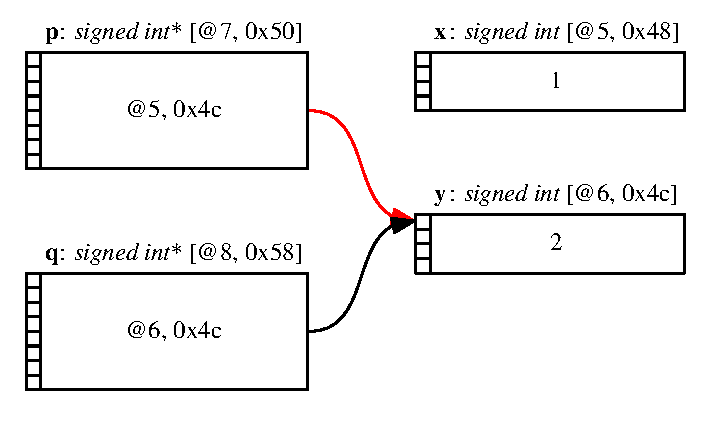
\includegraphics[width=0.5\textwidth]{provenance-basic-global-xy-memory.pdf}
\label{fig:pbweb-interface}
\vspace*{-2\baselineskip}
\end{wrapfigure}
%\end{figure*}

On the right is a provenance-semantics memory-state snapshot
(from the Cerberus GUI)
for \myfooexamplename{provenance_basic_global_xy.c},
%(identical in this case for PVI and PNVI),
just before the invalid access via \lstinline{p}, showing how the
provenance mismatch makes it UB: at the attempted access via
\lstinline{p}, its pointer-value address 0x4c is not 
%

All this is for the \emph{C abstract machine} as defined in the
standard: compilers might rely on provenance in their alias analysis and
optimisation, but one would not expect normal implementations to record
or manipulate provenance at runtime (though dynamic or static analysis
tools might, as might non-standard implementations such as CHERI
C). Provenances therefore do not have program-accessible runtime representations in the abstract
machine.  



\myparagraph{Can one construct out-of-bounds (by more than one) pointer values by pointer arithmetic?}
%
Consider the example below, where \lstinline{q} is transiently (more
than one-past) out of
bounds but brought back into bounds before being used for access. 
In ISO C, constructing such a pointer value is clearly stated to be undefined
behaviour~\cite[6.5.6p8]{c11}.
This can be captured using the
provenance of the pointer value to determine the relevant bounds.
\begin{wrapfigure}{r}{0.45\textwidth}
  \vspace*{-0.0\baselineskip}
{\renewcommand{\mylistingmargin}{2mm}\myqtexample{charon_tests/}{cheri_03_ii.c}{}}
  \vspace*{-1.0\baselineskip}
\end{wrapfigure}%
%
There are cases where such pointer arithmetic would go wrong on some
platforms (some now exotic), 
e.g.~where pointer arithmetic subtraction overflows, or if the
transient value is not aligned and only aligned values are
representable at the particular pointer type, or for hardware that does
 bounds checking, or where pointer arithmetic might wrap at values
less than the obvious word size (e.g.~``near'' or ``huge'' 8086 pointers).
%
However, transiently out-of-bounds pointer construction
seems to be common in practice.
%, as we see in \S\ref{sec:comp}, and 
%in \citeN{Chisnall:2015:BPA:2694344.2694367}. 
%
It may be desirable to make it implementation-defined 
whether such pointer construction is allowed. 
That would continue to permit implementations in which it would go
wrong to forbid it, but give a clear way for other implementations
to document that they do not exploit this UB in compiler optimisations
that may be surprising to programmers. Cerberus supports both
semantics, with a switch. 
%

\newpage

\myparagraph{Inter-object pointer arithmetic}
The first example in this section relied on guessing (and then
checking) the offset between two allocations.   What if one instead
calculates the offset, with pointer subtraction; should that let
one move between objects, as below?
In ISO C11, the \lstinline{q-p} is UB
(as a pointer subtraction between pointers to
\begin{wrapfigure}{r}{0.55\textwidth}
{\renewcommand{\mylistingmargin}{0mm}\myfooexample{charon_tests/}{pointer_offset_from_ptr_subtraction_global_xy.c}{}%
}
\vspace*{-0\baselineskip}
\end{wrapfigure}
different objects, which
in some abstract-machine executions are not one-past-related).
In a variant semantics that allows construction of more-than-one-past
pointers,  one would have to
to choose whether the \lstinline{*r=11} access is UB or not. 
%
The basic provenance semantics will forbid it, because \lstinline{r}
will retain the provenance of the \lstinline{x} allocation, but its
address is not in bounds for that. 
%
This is probably the most desirable semantics: we have found very few
example idioms that intentionally use inter-object pointer arithmetic,
and the freedom that forbidding it gives to alias analysis and
optimisation seems significant. 


\

\

\ 


\myparagraph{Pointer equality comparison and provenance}
%
A priori, pointer equality comparison (with \lstinline{==} or \lstinline{!=}) might be expected
to just compare their numeric addresses, but 
we observe GCC 8.1 -O2 sometimes
regarding two pointers
\begin{wrapfigure}{r}{0.55\textwidth}
{\renewcommand{\mylistingmargin}{0mm}\myfooexample{charon_tests/}{provenance_equality_global_xy.c}{}%
}
\vspace*{-0\baselineskip}
\end{wrapfigure}
with the same address but different provenance
as nonequal. Unsurprisingly, this happens in
some circumstances but not others, e.g.~if the test is pulled into a
simple separate function, but not if in a separate compilation unit.
To be conservative w.r.t.~current compiler behaviour, pointer
equality in the semantics should give false if the addresses are not equal, but 
nondeterministically (at each runtime occurrence) either take provenance into
account or not if the addresses are equal -- this specification looseness accommodating 
implementation variation. 
Alternatively, one could require numeric comparisons, which would be a
simpler semantics for programmers but force that GCC behaviour to be regarded as a 
bug.  Cerberus supports both options.
One might also imagine making it UB to compare pointers that are not strictly within
their original allocation~\cite{krebbers-phd}, but that would
break loops that test against a one-past pointer, or 
requiring equality to \emph{always} take provenance into account, but
that would require implementations to track provenance at runtime.

The current ISO C11 standard text is too strong here unless numeric
comparison is required: 6.5.9p6 says \emph{``Two
pointers compare equal {\bfseries{}if and only if} both are [...] or one is a
pointer to one past the end of one array object and the other is a
pointer to the start of a different array object that happens to
immediately follow the first array object in the address space''},
which requires such pointers to compare equal -- reasonable pre-DR260CR,
but debatable after it.

Pointer equality should not be confused with alias analysis: we could
require \lstinline{==} to return true for pointers with the same
address but different provenance, while still permitting alias
analysis to regard the two as distinct by making accesses via pointers
with the wrong provenance UB.





\myparagraph{Pointer relational comparison and provenance}
%
In ISO C (6.5.8p5), inter-object pointer relational comparison (with \lstinline{<}
etc.) is undefined behaviour.  Just as for inter-object pointer
subtraction,
there are platforms where this would go wrong, but there are also
substantial bodies of code that rely on it, e.g.~for lock orderings


It may be desirable to make it implementation-defined 
whether such pointer construction is allowed. 

\newpage

\section{Refining the basic provenance model to support pointer
  construction via casts, representation Accesses, etc.}\label{sec:refinemodel}

To support low-level systems programming, C provides many other ways
to construct and manipulate pointer values:
%
\begin{itemize}
\item 
casts of pointers to integer types and back, possibly with integer
arithmetic, e.g.~to force alignment, or to store information in unused
bits of pointers;

\item
copying pointer values with \lstinline{memcpy};

\item
manipulation of the representation bytes of pointers, e.g.~via user
code that copies them via \lstinline{char*} or \lstinline{unsigned char*} accesses;

\item
type punning between pointer and integer values; 

\item
I/O, using either \lstinline{fprintf}/\lstinline{fscanf} and
the \lstinline{%p} format,  \lstinline{fwrite}/\lstinline{fread} on
the pointer representation bytes, or pointer/integer casts and
integer I/O;

\item
copying pointer values with \lstinline{realloc};

\item
constructing pointer values that embody knowledge established from
linking, and from constants that represent the addresses of
memory-mapped devices. 
\end{itemize}
%
A satisfactory semantics has to address all these, together with the
implications on optimisation.   We define and explore several 
 alternatives:

\begin{itemize}
\item \textbf{PNVI-plain}: a semantics that does not track provenance via integers,
but instead, at integer-to-pointer cast points, checks whether the 
given address points within a live object and, if so, recreates the
corresponding provenance.  We explain in the next section why this is not as damaging to
optimisation as it may sound.

\item \textbf{PNVI-ae (PNVI exposed-address)}: a variant of PNVI that
  allows integer-to-pointer casts to recreate provenance only for
  provenances for which an address has previously been cast to
  integer. 

  \item \textbf{PNVI-ae-udi (PNVI exposed-address
    user-disambiguation)}: a further refinement of PNVI-ae that
supports casts of integers that are one-past an allocation.
This is the currently preferred option in the C memory object model
study group. 

\item \textbf{PVI}: a semantics that tracks provenance via integer computation,
associating a provenance with all integer values (not just pointer
values),
preserving provenance through integer/\break{}pointer casts, and making some
particular choices for the provenance results of integer and
pointer \lstinline{+}/\lstinline{-} integer operations;
or
\end{itemize}
We write PNVI-* for PNVI-plain, PNVI-ae, and PNVI-ae-udi.
The PNVI-plain and PVI semantics were described in the POPL 2019/N2311
paper.  PNVI-ae and PNVI-ae-udi have emerged from discussions in the C
memory object model study group. 


We also mention other variants of PNVI that seem less desirable:
\begin{itemize}
\item \textbf{PNVI-address-taken}: a variant that integer-to-pointer
  casts  to objects
whose address has been taken;  and
%\item \textbf{PNVI-escaped}: potential variants that
%additionally restrict to objects whose address has been taken and (in
%some sense) escaped; and
\item \textbf{PNVI-wildcard}: a variant that gives a ``wildcard''
provenance to the results of integer-to-pointer casts, delaying checks
to access time.
\end{itemize}
%


The PVI semantics, originally developed
informally in ISO WG14 working papers~\cite{N2090,N2263}, 
was motivated in part by 
the GCC documentation~\cite{gcc-arrays}:
\begin{quote}
\emph{``When casting from pointer to integer and back again, the
    resulting pointer must reference the same object as the original
    pointer, otherwise the behavior is undefined. That is, one may
    not use integer arithmetic to avoid the undefined behavior of
    pointer arithmetic as proscribed in C99 and C11 6.5.6/8.''}
\end{quote}
which presumes there is \emph{an} ``original'' pointer, and by experimental data for 
\lstinline{uintptr_t} analogues of the first test of \S\ref{sec:prov},
which suggested that GCC and ICC sometimes track provenance via
integers
(see \mytestlink{provenance_basic_using_uintptr_t_global_xy.c}{\lstinline{xy}} and
\mytestlink{provenance_basic_using_uintptr_t_global_yx.c}{\lstinline{yx}}
variants). 
%(\myfooexamplename{provenance_basic_using_uintptr_t_global_xy.c} and
%\myfooexamplename{provenance_basic_using_uintptr_t_global_yx.c}). 
However, discussions at the 2018 GNU Tools Cauldron suggest instead
that at least some key developers regard
the result of casts from integer types as potentially broadly
aliasing, at least in their GIMPLE IR, and such test results as long-standing
bugs in the RTL backend.

% Shifting to a provenance semantics that does not track provenance via
% integers would be a substantial simplification, in the definition of
% the semantics, in how easy it is for people to understand, and in the
% consequences for existing code (which might otherwise need additional
% annotations for exotic idioms).  That leads us to articulate and explore the various
% options above, to see which could be broadly acceptable.

\newpage

\section{Refining the basic provenance model: phenomena and examples}

\myparagraph{Pointer/integer casts}
The ISO standard (6.3.2.3) leaves conversions between pointer and integer types
almost entirely implementation-defined, except for conversion of
integer constant \texttt{0} and null pointers, and for the
\begin{wrapfigure}{r}{0.55\textwidth}
{\renewcommand{\mylistingmargin}{0mm}\myfooexample{charon_tests}{provenance_roundtrip_via_intptr_t.c}{}%
}
\vspace*{-2\baselineskip}
\end{wrapfigure}
optional \lstinline{intptr_t} and \lstinline{uintptr_t} types, for
which it guarantees that any \emph{``valid pointer to \lstinline{void}''} can
be converted and back, and that \emph{``the result will compare equal to the
original pointer''}.  As we have seen, in a post-DR260CR
provenance-aware semantics, \emph{``compare equal''} is not enough to
guarantee the two are interchangeable, which was clearly the intent of
that phrasing.  All variants of PNVI-* and PVI  support this, by 
reconstructing or preserving the original provenance respectively.

\ 

 
\myparagraph{Inter-object integer arithmetic}
Below is a \lstinline{uintptr_t} analogue of the \S\ref{sec:prov} example
\texttt{pointer\_offset\_from\_ptr\_subtraction\_global\_xy.c}, attempting to move between objects
with \lstinline{uintptr_t}
\begin{wrapfigure}{r}{0.55\textwidth}
{\renewcommand{\mylistingmargin}{0mm}\myfooexample{charon_tests}{pointer_offset_from_int_subtraction_global_xy.c}{}%
}
\vspace*{-2\baselineskip}
\end{wrapfigure}
arithmetic.
%
In PNVI-*, this has defined behaviour.  For PNVI-plain: the integer
values are pure integers, and at the \lstinline{int*} cast
the value of \lstinline{ux+offset} matches the address
of \lstinline{y} (live and of the right type), so the
resulting pointer value takes on the provenance of the \lstinline{y}
allocation.  For PNVI-ae and PNVI-ae-udi, the allocation to \lstinline{y}
is marked as \emph{exposed} at the cast of \lstinline{&y} to an
integer, and so the above is likewise permitted there. 

In PVI, this is UB. First,
the integer values of \lstinline{ux}
and \lstinline{uy} have the provenances of the allocations
of \lstinline{x} and \lstinline{y} respectively. Then 
\lstinline{offset} is a subtraction of two integer values with
non-equal single provenances; we define the result of such to have the
empty provenance.  Adding that empty-provenance result
to \lstinline{ux} preserves the original \lstinline{x}-allocation
provenance of the latter, as does 
the cast to \lstinline{int*}.
Then the final \lstinline{*p=11} access is via a pointer value whose
address is not consistent with its provenance.
%
 %
%
Similarly, PNVI-* allows
(contrary to current GCC/ICC O2) while PVI
forbids a \lstinline{uintptr_t} analogue of the
first test of \S\ref{sec:prov}, on the left below.
%\begin{wrapfigure}{r}{0.55\textwidth}



\begin{center}
  \begin{minipage}[t]{0.49\textwidth}
{\renewcommand{\mylistingmargin}{0mm}\myfooexample{charon_tests}{provenance_basic_using_uintptr_t_global_xy.c}{}%
}
\vspace*{-0\baselineskip}
\end{minipage}
  \begin{minipage}[t]{0.49\textwidth}
    {\renewcommand{\mylistingmargin}{0mm}\myfooexample{charon_tests}{pointer_offset_xor_global.c}{}%
}
  \end{minipage}
  \end{center}
Both choices are defensible here: PVI will permit more aggressive
alias analysis for pointers computed via integers (though those may be
relatively uncommon), while PNVI-* will
allow not just this test, which as written is probably not idiomatic
desirable C, but also the essentially identical XOR doubly linked list
idiom, using only one pointer per
node by storing the XOR of two, on the right above.  Opinions differ as to
whether that idiom matters for modern code. 

There are other real-world but rare cases of inter-object arithmetic,
e.g.~in
the implementations of Linux and FreeBSD per-CPU variables, in fixing
up pointers after a \lstinline{realloc}, and in dynamic linking
 (though
arguably some of these are not between C abstract-machine objects).
These are rare enough that it seems reasonable to require additional
source annotation, or some other mechanism, to prevent compilers
implicitly assuming that uses of such pointers as undefined. 


\myparagraph{Pointer provenance for pointer bit manipulations}
It is a standard idiom in systems code to use otherwise unused bits of
pointers: low-order bits for pointers known 
%
to be aligned,
\begin{wrapfigure}{r}{0.57\textwidth}
{\renewcommand{\mylistingmargin}{0mm}\myqtexample{charon_tests/}{provenance_tag_bits_via_uintptr_t_1.c}{http://www.cl.cam.ac.uk/users/pes20/cerberus/tests/provenance_tag_bits_via_uintptr_t_1.c.html}
}
\vspace*{-1.0\baselineskip}
\end{wrapfigure}
and/or
high-order bits beyond the addressable range.
The example on the right (which assumes \lstinline{_Alignof(int) >= 4}) 
does this: 
casting a pointer to \lstinline{uintptr_t} and back, using bitwise logical operations on the integer
value to store some tag bits. 

To allow this, we 
suggest that the set of unused bits for pointer types of each alignment
should be made implementation-defined.
In PNVI-* the intermediate value of \lstinline{q} will have empty
provenance, but the value of \lstinline{r} used for the access will 
re-acquire the correct provenance at cast time. 
In PVI we make the binary operations used here, combining an integer value that has some
provenance ID with a pure integer, preserve that provenance. 

(A separate question is the behaviour if the integer value with tag
bits set is converted back to pointer type.  In ISO the result is
implementation-defined, per 6.3.2.3p\{5,6\} and 7.20.1.4.)


\myparagraph{Algebraic properties of integer operations}
The PVI definitions of the provenance results of integer operations,
chosen to make the previous two examples respectively forbidden and
allowed, has an unfortunate consequence:  it makes those operations no
longer associative. Compare the examples below:

\

\begin{center}
{\renewcommand{\mylistingmargin}{0mm}\myfooexample{charon_tests}{pointer_arith_algebraic_properties_2_global.c}{}%
}
{\renewcommand{\mylistingmargin}{0mm}\myfooexample{charon_tests}{pointer_arith_algebraic_properties_3_global.c}{}%
}
\end{center}
\vspace*{-\baselineskip}
The latter is UB in PVI.
%\TODO{make example
%\url{http://www.open-std.org/jtc1/sc22/wg14/www/docs/n2263.htm#q12.-for-arithmetic-over-provenanced-integer-values-is-the-provenance-of-the-result-invariant-under-commutativity-and-under-plusminus-associativity}
%}.
It is unclear whether this would be acceptable
in practice, either for C programmers or for compiler optimisation.
One could conceivably switch to a PVI-multiple variant, allowing
provenances to be finite sets of allocation IDs.  That would allow the
\myfooexamplename{pointer_offset_from_int_subtraction_global_xy.c} example above, but perhaps too much else besides.
The PNVI-* models do not suffer from this problem.


\myparagraph{Copying pointer values with \lstinline{memcpy()}}
This clearly has to be allowed, and so, to make the results usable for
accessing memory without UB, \lstinline{memcpy()} and similar functions have to preserve the original
provenance.
%
\begin{wrapfigure}{r}{0.55\textwidth}
{\renewcommand{\mylistingmargin}{0mm}\myfooexample{charon_tests}{pointer_copy_memcpy.c}{}%
}
\vspace*{-2\baselineskip}
\end{wrapfigure}
%
%
The ISO C11 text does not explicitly address this (in a
pre-provenance semantics, before DR260, it did not need to).
One could do so by special-casing \lstinline{memcpy()} and similar
functions to preserve provenance,
but the following questions suggest less ad hoc approaches,
for PNVI-plain or PVI.  For PNVI-ae and PNVI-ae-udi, the best approach
is not yet clear.

\

\

\

\myparagraph{Copying pointer values bytewise, with user-\lstinline{memcpy}}
One of the key aspects of C is that it supports manipulation of object
representations, e.g.~as in the following naive user implementation of
a \lstinline{memcpy}-like function,
\begin{wrapfigure}{r}{0.57\textwidth}
{\renewcommand{\mylistingmargin}{0mm}\myfooexample{charon_tests/}{pointer_copy_user_dataflow_direct_bytewise.c}{http://www.cl.cam.ac.uk/users/pes20/cerberus/tests/pointer_copy_user_dataflow_direct_bytewise.c.html}%
}
\vspace*{-1.0\baselineskip}
\end{wrapfigure}
which constructs a pointer value from copied bytes. 
This too should be allowed.
PNVI-plain makes it legal: the representation
bytes have no
provenance, but when reading a pointer value from the
copied memory, the read will be from multiple representation-byte
writes.  We use essentially the same semantics for such reads as for
integer-to-pointer casts: checking at read-time that the address is
within a live object, and giving the result the corresponding
provenance. 
%
PNVI-ae and PNVI-ae-udi need additional machinery, not yet developed in
detail, to permit this.

\

\

\

\

\


One could:
\begin{enumerate}
\item Mark allocations as exposed whenever representation bytes of
  pointers to them are read, and use the same semantics for reads of
  pointer values from representation-byte writes as for
  integer-to-pointer casts. This is attractively simple, but also
  means that integer-to-pointer casts become permitted for all such
  allocations, perhaps over-liberally.
\item Record symbolically in the semantics of integer values what such
  representation-byte values are of the form ``byte $n$ of pointer
  value $v$'', or perhaps ``byte $n$ of pointer value of type $t$'', and allow reads of pointer values from
  representation-byte writes only for such.  This is more complex and
  rather ad hoc, arbitrarily restricting the integer computation that
  can be done on such bytes.
\end{enumerate}
%There may not be much reasonable
%code that would be sensitive to the distinctions between these, but there is some, e.g.~manipulations of pointers where one knows the high-order bytes
%are the same. This is important in some language runtimes,
%using 32- or 48-bit values for pointers in a 64-bit architecture.

As Lee observes [private communication], to make it legal for
compilers to replace user-memcpy by the library version, one might
want the two to have exactly the same semantics.  Though strictly
speaking that is a question about the compiler intermediate language
semantics, not C source semantics. 

PVI makes user-memcpy legal by regarding each 
byte (as an integer value) as having the provenance of the original
pointer, and the result pointer, being composed of representation
bytes of which at least one has that provenance and none have a conflicting provenance, as having the same.
%
%

Real \lstinline{memcpy()} implementations are more complex. The glibc \lstinline{memcpy()}\cite{glibc_memcpy}
involves copying byte-by-byte, as
above, and also
word-by-word and, using virtual memory manipulation, page-by-page.
Word-by-word copying is not permitted by the ISO standard, as it
violates the effective type rules, but we believe C2x should support
it for suitably annotated code. Virtual memory manipulation is outside our scope
at present. 


\myparagraph{Reading pointer values from byte writes in PNVI-*}
In all these provenance semantics, pointer values carry their
provenance unchanged, both while manipulated in expressions (e.g.~with pointer
arithmetic) and when stored or loaded as values of pointer type.
%
In the detailed semantics, memory contains abstract bytes rather than
general C language values, and so we record provenance in memory by attaching
a provenance to each abstract byte.  For pointer values stored by
single writes, this will usually be identical in each abstract byte of
the value.

However, in PNVI-*,
if one reads a pointer value that has been partially or completely
written by (integer) representation-byte writes, we use the same
semantics as for integer-to-pointer casts, reading the address and
reconstructing the associated provenance iff a live storage
instance covering that address exists (and, for PNVI-ae and
PNVI-ae-udi, if that instance has been exposed).
%
To determine whether a pointer value read is from a single write (and
thus should retain its original provenance when read), or from a combination of
representation byte writes and perhaps also a pointer value write (and
thus should use the integer-to-pointer cast semantics when read),
we also record, in each abstract byte, an optional pointer-byte index
(e.g.~in $0..7$ on an implementation with 8-byte pointer values). 
Pointer value writes will set these to the consecutive sequence
$0,1,..,7$, while other writes will clear them. 
%
For example, the code on the left below sets the fourth byte of
\lstinline{p} to \lstinline{0}. The memory state on the right, just
after the \lstinline{*q=2}, shows the pointer-byte indices of
\lstinline{p}, one of which has been cleared (shown as ?).  When the
value of \lstinline{p} is read (e.g.~in the \lstinline{q=p}), the fact
that there is not a consecutive sequence $0,1,..,7$ means that PNVI-*
will apply the integer-to-pointer cast semantics, here successfully
recovering the provenance \lstinline{@3} of the storage instance
\lstinline{x}.  Then the write of \lstinline{q} will itself have a
consecutive sequence (its pointer-byte indices are therefore
suppressed in the diagram).  Any non-pointer write overlapping the
footprint of \lstinline{p}, or any pointer write that overlaps that
footprint but does not cover it all, would remove the consecutive
sequence of indices.  
\begin{center}
  \begin{tabular}{cc}
{\begin{lstlisting}
int x=1;
int main() {
  int *p = &x;
  if (*((unsigned char*)&p+4)==0)
    *((unsigned char*)&p+4)=0;
  int *q = p;
  *q=2;
}
\end{lstlisting}}
&
\raisebox{-3cm}{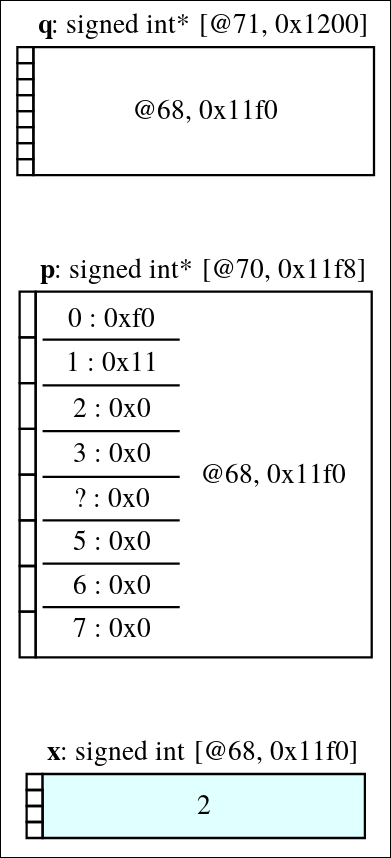
\includegraphics[width=0.2\textwidth]{pointer_byte.png}}
  \end{tabular}
  \end{center}
In PNVI-plain a representation-byte copy of a pointer value thus is
subtly different from a copy done at pointer type: the latter retains
the original provenance, while the former, when it is loaded, will
take on the provenance of whatever storage instance is live (and covers
its address) \emph{at load time}.  

The conditional in the example is needed to avoid UB: the semantics
does not constrain the allocation
address of \lstinline{x}, so there are executions in which byte 4 is
not \lstinline{0}, in which case the read of \lstinline{p} would have
a wild address and the empty provenance, and the write
\lstinline{*q=2} would flag UB. 

\newpage
\myparagraph{Pointer provenance for bytewise pointer representation manipulations}
To examine the possible semantics for pointer representation bytes
more closely, especially for PNVI-ae and PNVI-ae-udi, consider the
following.
As in
\myfooexamplename{provenance_tag_bits_via_uintptr_t_1.c}, it
manipulates the low-order bits of a pointer value, but now it
does so
by manipulating one of its representation bytes (as in
\myfooexamplename{pointer_copy_user_dataflow_direct_bytewise.c})
\begin{wrapfigure}{r}{0.67\textwidth}
%\begin{center}
%  \begin{minipage}[t]{0.49\textwidth}
{\renewcommand{\mylistingmargin}{0mm}\myfooexample{charon_tests}{provenance_tag_bits_via_repr_byte_1.c}{}%
}
\vspace*{-0\baselineskip}
%\end{minipage}
%\end{center}
  \vspace*{-1.0\baselineskip}
\end{wrapfigure}
instead of by casting to \lstinline{uintptr_t} and back. 
In PNVI-plain and PVI this will just work, respectively
reconstructing the original provenance and tracking it through the
(changed and unchanged) integer bytes.  But in PNVI-ae and
PNVI-ae-udi,
the address of \lstinline{x} has not been exposed by any
pointer-to-integer casts.  What should the semantics of the last reads
of the value of \lstinline{p}, from a combination of the original
\lstinline{p=&x} write and later integer byte writes, be?  

\

\

\

\

\

\

\

\

\ 



\myparagraph{Copying pointer values via encryption}
To more clearly delimit what idioms our proposals do and do not
allow, consider copying pointers via code that encrypts or compresses a block of
multiple pointers together, decrypting or uncompressing later.

In PNVI-plain, it would just work, in the same way as \lstinline{user_memcpy()}.
In PNVI-ae and PNVI-ae-udi, it would work if the pointer values are
cast to integer types, but if not, and they are encrypted by reading
their representation bytes, then for the models as currently stated it
would not work, just as for
\myfooexamplename{provenance_tag_bits_via_repr_byte_1.c}. 

It has been argued that pointer construction via \lstinline{intptr_t} and back via any
value-dependent identity function should be required to work.  That
would admit these, but defining that notion of ``value-dependent'' is
exactly what is hard in the concurrency thin-air problem~\cite{BMNPS2015},
and we do not believe that it is practical to make compilers respect dependencies in general.

In PVI, this involves exactly the same combination of distinct-provenance
values that (to prohibit inter-object arithmetic, and thereby enable
alias analysis) we above regard as having empty-provenance results.  
As copying pointers in this way  is a very rare idiom, one can argue
that  it is reasonable to require such
code to have additional annotations.

\newpage

\myparagraph{Copying pointer values via control flow} 
We
also have to ask whether a usable pointer can be constructed via
non-dataflow control-flow paths, e.g.~if testing
equality of an unprovenanced integer value against a valid pointer
permits the integer to be used as if it had the same provenance as the
pointer.  We do not believe that this is relied on in practice.
 For example, consider
exotic versions of
\lstinline{memcpy}
that make a control-flow choice on the
value of each bit or each byte, reconstructing each with constants in
each control-flow branch

\

\begin{center}
  \begin{minipage}[t]{0.49\textwidth}
{\renewcommand{\mylistingmargin}{0mm}\myfooexample{charon_tests}{pointer_copy_user_ctrlflow_bytewise_abbrev.c}{}%
}
\vspace*{-0\baselineskip}
\end{minipage}
  \begin{minipage}[t]{0.49\textwidth}
    {\renewcommand{\mylistingmargin}{0mm}\myfooexample{charon_tests}{pointer_copy_user_ctrlflow_bitwise.c}{}%
}
  \end{minipage}
  \end{center}
In PNVI-plain these would both work, while in PNVI-ae and PNVI-ae-udi
only the second would, as the first reads representation bytes rather
than casting the pointer value to integer. In PVI they would give
empty-provenance pointer values and hence UB.


\newpage
\myparagraph{Integer comparison and provenance}
If integer values have associated provenance, as in PVI, one has to ask whether
the result of an integer comparison should also be allowed to be provenance
dependent (\myfooexamplename{provenance_equality_uintptr_t_global_xy.c}).  
GCC did do so at one point, but it was regarded as a
bug and fixed (from 4.7.1 to 4.8).   We propose that the numeric
results of all operations on integers should be unaffected by the
provenances of their arguments. 
For PNVI-*, this question is moot. 


\myparagraph{Pointer provenance and union type punning}
Pointer values can also be constructed in C by type punning, e.g.~writing
a \lstinline{uintptr_t} union member and then reading it as a
pointer-type member
\begin{wrapfigure}{r}{0.45\textwidth}
  \vspace*{-0.0\baselineskip}
          {\renewcommand{\mylistingmargin}{0mm}\myfooexample{charon_tests/}{provenance_union_punning_2_global_xy.c}{}
          }
  \vspace*{-1.0\baselineskip}
\end{wrapfigure}%
The ISO standard says \emph{``the appropriate part of the object
representation of the value is reinterpreted as an object
representation in the new type''}, but says little about that
reinterpretation. %, and DR260 CR does not speak to the provenance of the
%result.
We propose that these reinterpretations be required to be
implementation-defined,
and, in PNVI-plain, that the
same integer-to-pointer cast semantics be used at such reads
(the latter does not match current ICC O2 behaviour). 

For PNVI-ae and PNVI-ae-udi, it's not clear what the best semantics
would be. 

For PVI, we propose that it be
implementation-defined whether the result preserves the original
provenance (e.g.~where they are the identity).

\

\

\

\

\


\

\

\

\

\



\myparagraph{Pointer provenance via IO}
Consider now pointer provenance flowing 
via IO, e.g.~writing the address of an object to a pipe or file and reading it
back in.
We have three versions: one using \lstinline{fprintf}/\lstinline{fscanf} and
the \lstinline{%p} format, one using \lstinline{fwrite}/\lstinline{fread} on
the pointer representation bytes, and one converting the pointer to
and from \lstinline{uintptr_t} and using
\lstinline{fprintf}/\lstinline{fscanf} on that value with the
\lstinline{PRIuPTR}/\lstinline{SCNuPTR} formats
(\myfooexamplename{provenance_via_io_percentp_global.c},
\myfooexamplename{provenance_via_io_bytewise_global.c}, and
\myfooexamplename{provenance_via_io_uintptr_t_global.c})
The first gives a syntactic indication of a potentially
escaping pointer value, while the others (after preprocessing) do
not. 
% SKIP FOR SPACE
%Giving just the first in full:
%
%\myqtexample{charon_tests/}{provenance_via_io_percentp_global.c}{http://www.cl.cam.ac.uk/users/pes20/cerberus/tests/provenance_via_io_percentp_global.c.html}
%
Somewhat exotic though they are, these idioms are used in practice: in 
graphics code for
serialisation/deserialisation (using \lstinline{%p}), 
in xlib (using \lstinline{SCNuPTR}), and in debuggers.

In the ISO standard, the text for \lstinline{fprintf} and
\lstinline{scanf} for \lstinline{%p} says that this should work: \emph{``If
  the input item is a value converted earlier during the same program
  execution, the pointer that results shall compare equal to that
  value; otherwise the behavior of the \texttt{\%p} conversion is
  undefined''}  (again construing the pre-DR260 ``compare equal'' as implying
  the result should be usable for access),
and the text for \lstinline{uintptr_t} and the presence of
\lstinline{SCNuPTR} in \lstinline{inttypes.h} weakly implies the same there.

But then what can compiler alias analyses assume about such a pointer
read?  
In PNVI-plain, this is simple: at \lstinline{scanf}-time, for the \lstinline{%p}
version, or when a pointer is read from memory written by the
other two, we can do a runtime check and potential acquisition of
provenance exactly like an integer-to-pointer cast.
%

In PNVI-ae and PNVI-ae-udi, for the \lstinline{%p}
  case we could mark the associated storage instance as exposed by the
  output, and
  use
  the same semantics as integer-to-pointer casts on the input.
  The \lstinline{uintptr_t} case would also work straightforwardly.
  However, the representation-byte output and input is problematic,
  just as for bytewise memcpy above.   


For PVI, there are several options, none of which seem ideal:
we could use a PNVI-like semantics, but that would be
stylistically inconsistent with the rest of PVI; or (only for the first) we could restrict that to provenances that have been output via
\lstinline{%p}), or
we could require new programmer annotation, at output and/or
input points, to constrain alias analysis. 



\myparagraph{Pointers from device memory and linking}
In practice, concrete memory addresses or relationships between them
sometimes are determined and relied on by programmers, 
in implementation-specific ways.
%
Sometimes these are simply concrete absolute addresses which will
never alias C stack, heap, or program memory,
e.g.~those of particular memory-mapped devices
in an embedded system.
%
Others are absolute addresses and relative layout of program code and
data, usually involving one or more \emph{linking} steps.
For example, platforms may lay out 
certain regions of memory so as to obey
particular relationships, e.g.~in a commodity operating system
where high addresses are used for kernel mappings,
initial stack lives immediately below the arguments
passed from the operating system, and so on.
%
The details of linking and of platform memory maps
are outside the scope of ISO C, but real C code may embody knowledge of them.
Such code might be as simple as casting a
platform-specified address, represented as an integer literal,
to a pointer. It might be more subtle,
such as assuming that one object directly follows another in memory---the
programmer having established
this property at link time (perhaps by a custom linker script).
It is necessary to preserve the legitimacy of such C code,
so that compilers may not view such memory accesses as undefined
behaviour, even with increasing link-time optimisation. 

We leave the design of exactly what escape-hatch mechanisms are
needed here as an open
problem.  For memory-mapped devices, one could simply posit
implementation-defined ranges of such memory which are guaranteed not
to alias C objects.  The more general linkage case is more
interesting, but well outside current ISO C.
%
The tracking of provenance through embedded assembly is similar.



\myparagraph{Pointers from allocator libraries}
Our semantics special-cases \lstinline{malloc} and the related
functions, by giving their results fresh provenances.  This is
stylistically consistent with the ISO text, which also special-cases
them, but it would be better for C to support a general-purpose
annotation, to let both \lstinline{stdlib} implementations and other
libraries return pointers that are treated as having fresh provenance
outside (but not inside) their abstraction boundaries.


\TODO{PNVI-ae and PNVI-ae-udi considered up to here only}


\section{Implications of Provenance Semantics for Optimisations}\label{sec:opt}

In an ideal world, a memory object semantics for C would be consistent
with all existing mainstream code usage and compiler behaviour.  In practice, we
suspect that (absent a precise standard) these have
diverged too much for that, making some compromise required. 
As we have already seen, the PNVI semantics would make some currently
observed GCC and ICC behaviour unsound, though at
least some key GCC developers already regard that behaviour as a
longstanding unfixed bug, due to the lack of integer/pointer type
distinctions in RTL.
%The performance and compiler change cost of
%adapting compilers to either PNVI or PVI is an important question, but
%one principally for the compiler teams to answer. 
%
We now consider some other important cases, by example. 


\myparagraph{Optimisation based on equality tests}
Both provenance semantics let \lstinline{p==q} hold in some cases
where \lstinline{p} and \lstinline{q} are not interchangeable. 
As \citeN{oopslaTwin} observe in the LLVM 
IR context, that
may limit optimisations such as GVN (global value numbering) based on
pointer equality tests.
PVI suffers from the same problem also for integer comparisons,
wherever the integers might have been cast from pointers and eventually be
cast back. This may be more serious. 



\myparagraph{Can a function argument alias local variables of the
function?}
In general one would like this to be forbidden, to let optimisation
assume its absence.  Consider first the
example below, where
\begin{wrapfigure}{r}{0.4\textwidth}
\vspace*{-0.25\baselineskip}
{\renewcommand{\mylistingmargin}{0mm}\myfooexample{charon_tests/}{pointer_from_integer_1pg.c}{}%{pointer_from_integer_1i.c}%
}
\vspace*{-0.75\baselineskip}
\end{wrapfigure}
 \lstinline{main()} guesses the address of \lstinline{f()}'s local
 variable, passing it in as a pointer, and \lstinline{f()} checks it
 before using it for an access.
Here we see, for example, GCC -O0 optimising away the \lstinline{if} and
the write \lstinline{*p=7}, even in executions where the \lstinline{ADDRESS_PFI_1PG}
constant is the same as the \lstinline{printf}'d address
 of \lstinline{j}. 
%
We believe that compiler behaviour should be permitted, and hence that
this program should be deemed to have UB --- or, in other words, that
code should not normally be allowed to rely on implementation facts about the
allocation addresses of C variables.  The PVI semantics flags UB
for the simple reason that \lstinline{j} is created with the empty
provenance, and hence \lstinline{p} inherits that.  The PNVI semantics
also deems this to be UB, because at the point of
the \lstinline{(int*)i} cast the \lstinline{j} allocation does not yet
exist, so the cast gives a pointer with empty provenance; any
execution that goes into the \lstinline{if} would thus flag UB. 

\



\begin{wrapfigure}{r}{0.4\textwidth}
\vspace*{-0.25\baselineskip}
{\renewcommand{\mylistingmargin}{0mm}\myfooexample{charon_tests/}{pointer_from_integer_1ig.c}{}%{pointer_from_integer_1i.c}%
}
\vspace*{-0.75\baselineskip}
\end{wrapfigure}
Varying to do the cast to \lstinline{int*}
in \lstinline{f()} instead of \lstinline{main()}, passing in an
integer \lstinline{i}
instead of a pointer
this remains UB in PVI, but in PNVI becomes defined, as \lstinline{j}
exists at the point when the abstract machine does
the \lstinline{(int*)i} cast.
At present we do not see any strong reason why making this defined would not be
acceptable --- it amounts to requiring compilers to be conservative
for the results of integer-to-pointer casts where they cannot see the
source of the integer, which we imagine to be a rare case --- but this
does not match current O2 or O3 compilation for GCC, Clang, or ICC.

\

\

\

\

\

\

\newpage

\myparagraph{Allocation-address nondeterminism}
Note that both of the previous examples take the address
of \lstinline{j} to guard their \lstinline{*p=7} accesses.
Removing the conditional guards gives tests that one would surely like
to forbid

\

\begin{center}
  \begin{minipage}[t]{0.49\textwidth}
{\renewcommand{\mylistingmargin}{0mm}\myfooexample{charon_tests}{pointer_from_integer_1p.c}{}%
}
\vspace*{-0\baselineskip}
\end{minipage}
  \begin{minipage}[t]{0.49\textwidth}
    {\renewcommand{\mylistingmargin}{0mm}\myfooexample{charon_tests}{pointer_from_integer_1i.c}{}%
}
  \end{minipage}
  \end{center}
Both are forbidden in PVI for the same reason as before, and the first
is forbidden in PNVI again because \lstinline{j} does not exist at the
cast point.  

But the second forces us to think about how much allocation-address
nondeterminism should be quantified over in the basic definition of
undefined behaviour. For evaluation-order and concurrency
nondeterminism, one would normally say that if there exists any execution
that flags UB, then the program as a whole has UB (for the moment
ignoring UB that occurs only on some paths following I/O input, which
is another important question that the current ISO text does not address).  

This view of UB seems to be unfortunate but inescapable. 
If one looks just at a single execution, then 
 (at least between input points) we cannot
temporally bound the effects of an UB, because compilers can and do
re-order code w.r.t.~the C abstract machine's sequencing of
computation.  In other words, UB may be flagged at some specific point
in an abstract-machine trace, but its consequences on the observed
implementation behaviour might happen much earlier (in practice,
perhaps not very much earlier, but we do not have any good way of
bounding how much).
%
But then if one execution might have UB, and hence exhibit (in an
implementation) arbitrary observable behaviour, then anything the
standard might say about any other execution is irrelevant, because it
can always be masked by that arbitrary observable behaviour.

Accordingly, our semantics nondeterministically chooses an arbitrary
address for each allocation, subject only to alignment and no-overlap
constraints (ultimately one would also need to build in constraints
from programmer linking commands).  Then in PNVI, the \lstinline{..._1i.c} example is UB because, even
though there is one execution in which the guess is correct, there is
another (in fact many others) in which it is not. In those, the cast
to \lstinline{int*} gives a pointer with empty provenance, so the
access flags UB --- hence the whole program is UB, as desired.



\myparagraph{Can a function access local variables of its parent?}
This too should be forbidden in general. 
The example on the left below is forbidden by PVI, again for the simple reason that
 \lstinline{p}
has the empty provenance, and 

\

\begin{center}
  \begin{minipage}[t]{0.49\textwidth}
{\renewcommand{\mylistingmargin}{5mm}\vspace*{-0.25\baselineskip}\mycerbexample{charon_tests/}{pointer_from_integer_2.c}{}{pointer_from_integer_2.c}\vspace*{-0.5\baselineskip}%
}
\vspace*{-0\baselineskip}
\end{minipage}
  \begin{minipage}[t]{0.49\textwidth}
{\renewcommand{\mylistingmargin}{5mm}\vspace*{-0.25\baselineskip}\mycerbexample{charon_tests/}{pointer_from_integer_2g.c}{}{pointer_from_integer_2g.c}\vspace*{-0.5\baselineskip}%
}
\vspace*{-0\baselineskip}
  \end{minipage}
  \end{center}
%
%
by PNVI by allocation-address
nondeterminism, as there exist abstract-machine
executions in which the guessed address
is wrong. 
%
One cannot guard the access within \lstinline{f()}, as
the address of \lstinline{j} is not available there.  Guarding the
call to \lstinline{f()} with 
%\makebox[0.4\textwidth][l]{
\lstinline{if ((uintptr_t)&j == ADDRESS_PFI_2)} %}
(\mycerbexamplename{pointer_from_integer_2g.c}{pointer_from_integer_2g.c})
again makes the example well-defined in PNVI, as the address is
correct and \lstinline{j} exists at the \lstinline{int*} cast point,
but notice again that the
guard necessarily involves \lstinline{&j}. 
This does not match current Clang at O2 or O3, which print \lstinline{j=5}.

\myparagraph{The PNVI-address-taken, PNVI-escaped, and PNVI-wildcard alternatives}
An obvious refinement to PNVI is to restrict integer-to-pointer casts
to recover the provenance only of objects that have had their address
taken, recording that in the memory state.  
Perhaps surprisingly, that seems not to make much difference to the
allowed tests, because the tests one might write tend to already be UB due
to allocation-address nondeterminism, or to already take the address
of an object to use it in a guard.  PNVI-address-taken has the conceptual advantage of
identifying these UBs without requiring examination of multiple
executions, but the disadvantage that whether an address has been
taken is a fragile syntactic property, e.g.~not preserved
by dead code elimination.  One can also restrict further, to addresses
that have in some sense escaped, but precisely defining a particular
such sense is complex and somewhat arbitrary. 
A rather different model is to make the results of integer-to-pointer
casts have a ``wildcard'' provenance, deferring the check that the
address matches a live object from cast-time to access-time.  This
would make \mycerbexamplename{pointer_from_integer_1pg.c}{pointer_from_integer_1pg.c} defined,
which is surely not desirable. 

\myparagraph{The problem with lost address-takens and escapes}
Our PVI proposal allows computations that erase the numeric
value (and hence a concrete view of the ``semantic dependencies'') of a
pointer, but retain provenance.  This makes examples like that below
[Richard Smith, personal communication],
in which the code correctly guesses an allocation address (which has
the empty provenance) and adds that to a zero-valued quantity (with
the correct provenance), 
allowed in PVI.  We emphasise that we do not think it
especially desirable to allow such examples; this is just a
consequence of choosing a straightforward provenance-via-integer semantics that
allows the bytewise copying and the bitwise manipulation of pointers
above.  In other words, it is not clear how it could be forbidden
simply in PVI.

%\myqtexample{charon_tests/}{provenance_lost_escape_2.c}{http://www.cl.cam.ac.uk/users/pes20/cerberus/tests/provenance_lost_escape_2.c.html}
%
\begin{wrapfigure}{r}{0.67\textwidth}
{\renewcommand{\mylistingmargin}{0mm}\vspace*{-0.0\baselineskip}
\mycerbexample{charon_tests/}{provenance_lost_escape_1.c}{http://www.cl.cam.ac.uk/users/pes20/cerberus/tests/provenance_lost_escape_1.c.html}{provenance_lost_escape_1.c}
\vspace*{-1.5\baselineskip}
}
\end{wrapfigure}
However, in implementations some algebraic optimisations may be done before alias
analysis, %---in particular, in LLVM, algebraic optimisations are--- 
and those optimisations might erase the  \lstinline{&x}, replacing it and
all the calculation of \lstinline{i3} by \lstinline{0x0} (a similar example would have \lstinline{i3 = i1-i1}).  
But then alias analysis would be unable to see that \lstinline{*q} could access
\lstinline{x}, and so report that it could not, and hence enable
subsequent optimisations
that are unsound w.r.t.~PVI for this case.  The basic point is that whether a
variable has its address taken or escaped in the source language is
not preserved by optimisation.
%
A possible solution, which would need some implementation work for
implementations that do track provenance through integers, but
perhaps acceptably so, would be to require those initial optimisation
passes to record the address-takens involved in computations they erase, so
that that could be passed in explicitly to alias analysis.
%
In contrast to the difficulties of preserving dependencies to avoid
thin-air concurrency, this does not forbid optimisations that remove
dependencies; it merely requires them to describe what they do.

In PNVI, the example is also allowed, but for a simpler reason that is
not affected by such integer optimisation: the object exists at
the \lstinline{int*} cast.  Implementations that  take a conservative view of all pointers
formed from integers  would automatically be sound w.r.t.~this. At
present ICC is not, at O2 or O3.

%

\myparagraph{Should PNVI allow one-past integer-to-pointer casts?}
For PNVI, one has to choose whether an integer that is one-past a live
object (and not strictly within another) can be cast to a pointer with valid provenance,
or whether this should give an empty-provenance pointer value. 
Lee observes that the latter may be necessary to make some
optimisation sound [personal communication], and we imagine that this is
not a normal idiom in practice, so we follow the stricter semantics here. 


\myparagraph{Summary of pros and cons}
Both semantics handle many cases as one would desire.
Both suffer from the non-interchangeability of pointers that have
compared equal (with \lstinline{==}) and PVI also from the same
problem for integers.
PVI suffers from the loss of algebraic properties of integer
arithmetic operations, the difficulty of accommodating pointer I/O,
and the problem with lost address-takens and escapes.   PNVI makes some currently
observable compiler behaviours
unsound, though at least for GCC some of these are viewed by some
developers as buggy in any case. 
PNVI is considerably simpler to define and explain than PVI, and on
balance we think PNVI is preferable. 


% % SKIP THIS, AS NO SPACE
% \section{Related pointer semantics questions}\label{sec:relatedp}
% Here we highlight three other questions about C pointer semantics, not
% provenance-related.
% 
% \myparagraph{Can \texttt{intptr\_t} arithmetic be used to mimic
%   pointer arithmetic?}
% This example does intra-object pointer arithmetic, to move
% between array elements, but at \lstinline{uintptr_t} type.
% %Example adapted from Martin Sebor mail (WG14):
% It is debatable
% \begin{wrapfigure}{r}{0.5\textwidth}
%   \vspace*{-1.0\baselineskip}
% {\renewcommand{\mylistingmargin}{5mm}\myqtexample{charon_tests/}{pointer_arithmetic_at_intptr_t_1.c}{}}
%   \vspace*{-1.0\baselineskip}
% \end{wrapfigure}%
% whether this should be allowed: the ISO text is
% unclear,
% and some WG14 members argue not, but it seems to be a common idiom
% in systems code. Our semantics allows it.
% %
% If one wanted to forbid it, that could be done by recording the original address
% of a pointer value at any pointer-to-integer casts, carrying that (not
% just the provenance) as ghost state with the pointer value, and allowing
% only integer-to-pointer casts that preserve the original address to preserve provenance.
% 
% 
% 
% 
% \myparagraph{Can pointers be used in non-access ways after the
%   lifetime of their original object?}
% In ISO, \emph{``The value of a pointer becomes indeterminate when
%  the object it points to (or just past) reaches the end of its
%  lifetime.''}  (6.4.2p2).
% This side-effect of lifetime end on \emph{all} pointer values that point to the object,
% wherever they may be in the abstract-machine state, is a highly unusual
% aspect of C when compared with other programming language definitions. 
% %
% % Note that there is no analogue of this for pointers to objects stored
% % within a \lstinline{malloc()}'d region when those objects are
% % overwritten (with a strong update) with something of a different type,
% % so this is not sufficient to maintain the invariant that all extant
% % pointer values point to something live of the appropriate type.
% %
% In practice the situation is less clear: some debugging environments
% null out pointers on \lstinline{free()} (though
% presumably not other pointers to the same object), but 
% several respondents suggest that checking equality
% %(with \lstinline{==} or \lstinline{!=})
%  against a pointer to an object whose
% lifetime has ended is used and is supported by implementations.
% %
% Here, again to bring ISO in line with common practice, and to prevent surprising compiler optimisations
% exploiting this UB, we suggest it be made implementation-defined or
% switchable in the standard whether pointer values become indeterminate
% at lifetime-end.






%% Bibliography

\makeatletter
% undo PS list hacks for bib
\setlength\labelsep{4pt}
\setlength{\@ACM@labelwidth}{6.5pt}
\makeatother
\bibliography{csembib-fullnames}



\end{document}
